
\documentclass[11pt,compress,t,notes=noshow, xcolor=table]{beamer}
\usepackage[]{graphicx}\usepackage[]{color}
% maxwidth is the original width if it is less than linewidth
% otherwise use linewidth (to make sure the graphics do not exceed the margin)
\makeatletter
\def\maxwidth{ %
  \ifdim\Gin@nat@width>\linewidth
    \linewidth
  \else
    \Gin@nat@width
  \fi
}
\makeatother

\definecolor{fgcolor}{rgb}{0.345, 0.345, 0.345}
\newcommand{\hlnum}[1]{\textcolor[rgb]{0.686,0.059,0.569}{#1}}%
\newcommand{\hlstr}[1]{\textcolor[rgb]{0.192,0.494,0.8}{#1}}%
\newcommand{\hlcom}[1]{\textcolor[rgb]{0.678,0.584,0.686}{\textit{#1}}}%
\newcommand{\hlopt}[1]{\textcolor[rgb]{0,0,0}{#1}}%
\newcommand{\hlstd}[1]{\textcolor[rgb]{0.345,0.345,0.345}{#1}}%
\newcommand{\hlkwa}[1]{\textcolor[rgb]{0.161,0.373,0.58}{\textbf{#1}}}%
\newcommand{\hlkwb}[1]{\textcolor[rgb]{0.69,0.353,0.396}{#1}}%
\newcommand{\hlkwc}[1]{\textcolor[rgb]{0.333,0.667,0.333}{#1}}%
\newcommand{\hlkwd}[1]{\textcolor[rgb]{0.737,0.353,0.396}{\textbf{#1}}}%
\let\hlipl\hlkwb

\usepackage{framed}
\makeatletter
\newenvironment{kframe}{%
 \def\at@end@of@kframe{}%
 \ifinner\ifhmode%
  \def\at@end@of@kframe{\end{minipage}}%
  \begin{minipage}{\columnwidth}%
 \fi\fi%
 \def\FrameCommand##1{\hskip\@totalleftmargin \hskip-\fboxsep
 \colorbox{shadecolor}{##1}\hskip-\fboxsep
     % There is no \\@totalrightmargin, so:
     \hskip-\linewidth \hskip-\@totalleftmargin \hskip\columnwidth}%
 \MakeFramed {\advance\hsize-\width
   \@totalleftmargin\z@ \linewidth\hsize
   \@setminipage}}%
 {\par\unskip\endMakeFramed%
 \at@end@of@kframe}
\makeatother

\definecolor{shadecolor}{rgb}{.97, .97, .97}
\definecolor{messagecolor}{rgb}{0, 0, 0}
\definecolor{warningcolor}{rgb}{1, 0, 1}
\definecolor{errorcolor}{rgb}{1, 0, 0}
\newenvironment{knitrout}{}{} % an empty environment to be redefined in TeX

\usepackage{alltt}
\newcommand{\SweaveOpts}[1]{}  % do not interfere with LaTeX
\newcommand{\SweaveInput}[1]{} % because they are not real TeX commands
\newcommand{\Sexpr}[1]{}       % will only be parsed by R
\newcommand{\xmark}{\ding{55}}%


\usepackage[english]{babel}
\usepackage[utf8]{inputenc}

\usepackage{dsfont}
\usepackage{verbatim}
\usepackage{amsmath}
\usepackage{amsfonts}
\usepackage{amssymb}
\usepackage{bm}
\usepackage{csquotes}
\usepackage{multirow}
\usepackage{longtable}
\usepackage{booktabs}
\usepackage{enumerate}
\usepackage[absolute,overlay]{textpos}
\usepackage{psfrag}
\usepackage{algorithm}
\usepackage{algpseudocode}
\usepackage{eqnarray}
\usepackage{arydshln}
\usepackage{tabularx}
\usepackage{placeins}
\usepackage{tikz}
\usepackage{setspace}
\usepackage{colortbl}
\usepackage{mathtools}
\usepackage{wrapfig}
\usepackage{bm}
\usepackage{amsmath}
\usepackage{pifont}
\usepackage{xcolor} %colored math symbols

\usetikzlibrary{shapes,arrows,automata,positioning,calc,chains,trees, shadows}
\tikzset{
  %Define standard arrow tip
  >=stealth',
  %Define style for boxes
  punkt/.style={
    rectangle,
    rounded corners,
    draw=black, very thick,
    text width=6.5em,
    minimum height=2em,
    text centered},
  % Define arrow style
  pil/.style={
    ->,
    thick,
    shorten <=2pt,
    shorten >=2pt,}
}

\usepackage{subfig}

% Defines macros and environments
\usepackage{../../style/lmu-lecture}


\let\code=\texttt
\let\proglang=\textsf

\setkeys{Gin}{width=0.9\textwidth}

\setbeamertemplate{frametitle}{\expandafter\uppercase\expandafter\insertframetitle}

\usepackage{bbm}
% basic latex stuff
\newcommand{\pkg}[1]{{\fontseries{b}\selectfont #1}} %fontstyle for R packages
\newcommand{\lz}{\vspace{0.5cm}} %vertical space
\newcommand{\dlz}{\vspace{1cm}} %double vertical space
\newcommand{\oneliner}[1] % Oneliner for important statements
{\begin{block}{}\begin{center}\begin{Large}#1\end{Large}\end{center}\end{block}}


%new environments
\newenvironment{vbframe}  %frame with breaks and verbatim
{
 \begin{frame}[containsverbatim,allowframebreaks]
}
{
\end{frame}
}

\newenvironment{vframe}  %frame with verbatim without breaks (to avoid numbering one slided frames)
{
 \begin{frame}[containsverbatim]
}
{
\end{frame}
}

\newenvironment{blocki}[1]   % itemize block
{
 \begin{block}{#1}\begin{itemize}
}
{
\end{itemize}\end{block}
}

\newenvironment{fragileframe}[2]{  %fragile frame with framebreaks
\begin{frame}[allowframebreaks, fragile, environment = fragileframe]
\frametitle{#1}
#2}
{\end{frame}}


\newcommand{\myframe}[2]{  %short for frame with framebreaks
\begin{frame}[allowframebreaks]
\frametitle{#1}
#2
\end{frame}}

\newcommand{\remark}[1]{
  \textbf{Remark:} #1
}


\newenvironment{deleteframe}
{
\begingroup
\usebackgroundtemplate{
\includegraphics[width=\paperwidth,height=\paperheight]{../style/color/red.png}}
 \begin{frame}
}
{
\end{frame}
\endgroup
}
\newenvironment{simplifyframe}
{
\begingroup
\usebackgroundtemplate{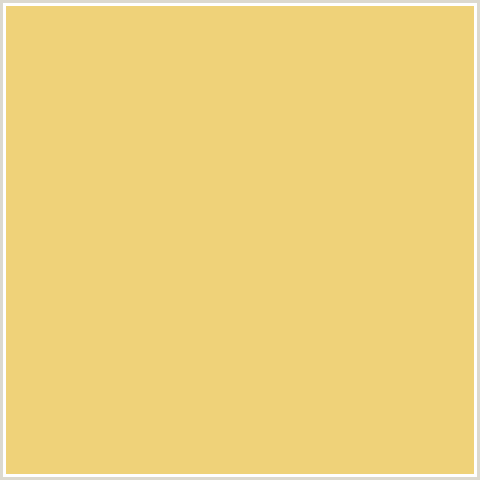
\includegraphics[width=\paperwidth,height=\paperheight]{../style/color/yellow.png}}
 \begin{frame}
}
{
\end{frame}
\endgroup
}\newenvironment{draftframe}
{
\begingroup
\usebackgroundtemplate{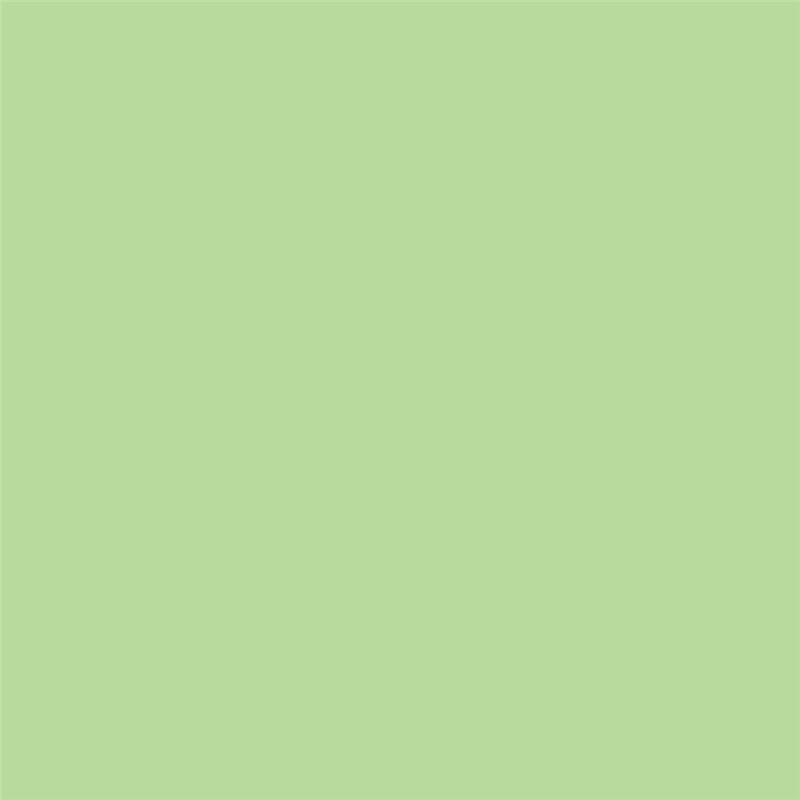
\includegraphics[width=\paperwidth,height=\paperheight]{../style/color/green.jpg}}
 \begin{frame}
}
{
\end{frame}
\endgroup
}
% https://tex.stackexchange.com/a/261480: textcolor that works in mathmode
\makeatletter
\renewcommand*{\@textcolor}[3]{%
  \protect\leavevmode
  \begingroup
    \color#1{#2}#3%
  \endgroup
}
\makeatother


\input{../../latex-math/basic-math}
\input{../../latex-math/basic-ml}
\input{../../latex-math/ml-nn}

\newcommand{\titlefigure}{plots/moderncnn/residual-block.png}
%modify picture
\newcommand{\learninggoals}{
  \item GoogleNet
  \item ResNet
  \item DenseNet
  \item U-Net
}

\title{Deep Learning}
\date{}



\begin{document}

\lecturechapter{Modern Architectures - II}
\lecture{I2DL}
%%%%%%%%%%%%%%%%%%%%%%%%%%%%%%%%%%%%%%%%%%%%%%%%%%%%%%%%%%%%%%%%%%


%%%%%%%%%%%%%%%%%%%%%%%%%%%%%%%%%%%%%%%%%%%%%%%%%%%%%%%%%%%%%%%%%%
\section{GoogLeNet}


\begin{vbframe}{Inception modules}
    \begin{itemize}
        \item The Inception block is equivalent to a subnetwork with four paths. 
        \item It extracts information in parallel through convolutional layers of different window shapes and max-pooling layers.  
        \item $1 \times 1$ convolutions reduce channel dimensionality on a per-pixel level. Max-pooling reduces the resolution.
    \end{itemize}
  \begin{figure}
    \centering
      \scalebox{0.75}{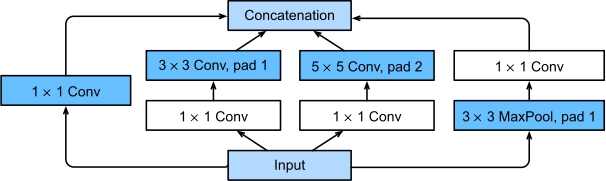
\includegraphics{plots/moderncnn/inception.png}}
    \caption{Inception Block (Dive into Deep Learning).}
  \end{figure}
        \end{vbframe}


\begin{vbframe}{GoogLeNet Architecture}
    \begin{itemize}
        \item GoogLeNet connects multiple well-designed Inception blocks with other layers in series. 
        \item The ratio of the number of channels assigned in the Inception block is obtained through a large number of experiments on the ImageNet dataset.
        \item GoogLeNet, as well as its succeeding versions, was one of the most efficient models on ImageNet, providing similar test accuracy with lower computational complexity.
    \end{itemize}
    \framebreak
    
  \begin{figure}
  \centering
    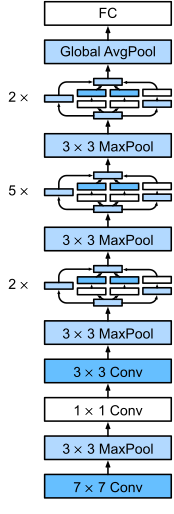
\includegraphics[width=2cm]{plots/moderncnn/inception-full.png}
    \caption{The GoogLeNet architecture (Dive into Deep Learning).}
  \end{figure}
    
\end{vbframe}

%%%%%%%%%%%%%%%%%%%%%%%%%%%%%%%%%%%%%%%%%%%%%%%%%%%%%%%%%%%%%%%%%%

\section{Residual Networks (ResNet)}

%\subsection{Residual Block}

\begin{vbframe}{Residual Block (Skip connections)}

Problem setting: theoretically, we could build infinitely deep architectures as the net should learn to pick the beneficial layers and skip those that do not improve the performance automatically.

 \begin{figure}
  \centering
    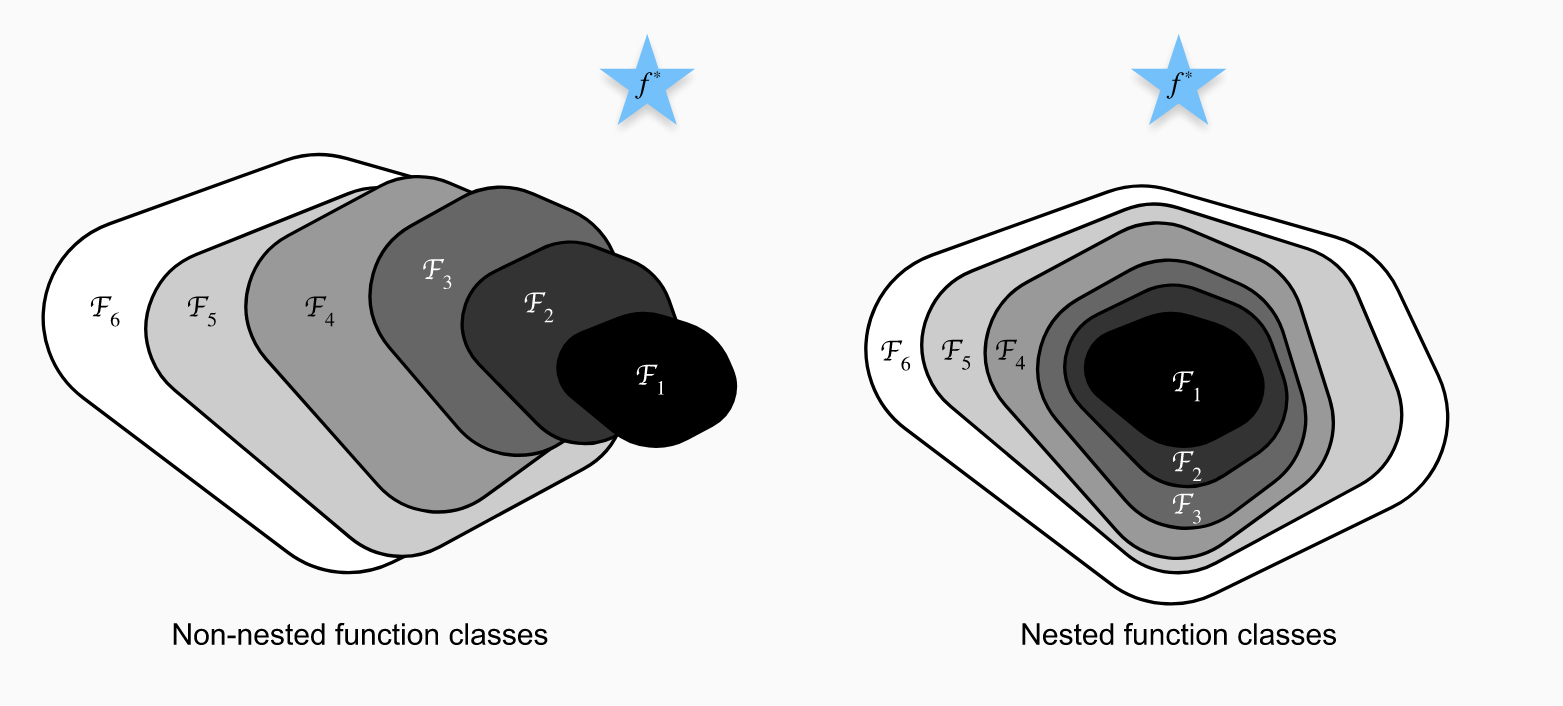
\includegraphics[width=8cm]{plots/moderncnn/resnet_problem.png}
    \caption{For non-nested function classes, a larger function class does not guarantee to get closer to the “truth” function ($\mathcal{F}*$). This does not happen in nested function classes (Dive into Deep Learning).}
  \end{figure}



    \begin{itemize}
        \item But: this skipping would imply learning an identity mapping $\xv = \mathcal{F}(\xv)$. It is very hard for a neural net to learn such a 1:1 mapping through the many non-linear activations in the architecture.
        \item Solution: offer the model explicitly the opportunity to skip certain layers if they are not useful.
        \item Introduced in \textit{He et. al , 2015} and motivated by the observation that stacking evermore layers increases the test- as well as the train-error ($\neq$ overfitting).
    \end{itemize}
\framebreak
 
 \begin{figure}
  \centering
    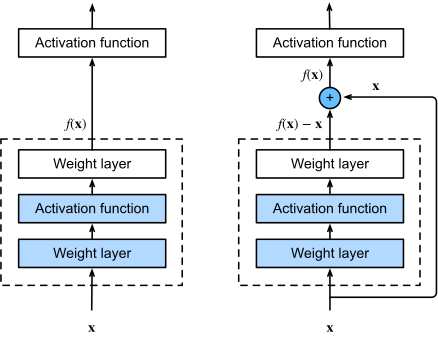
\includegraphics[width=6cm]{plots/moderncnn/residual-block.png}
    \caption{A regular block (left) and a residual block (right) (Dive into Deep Learning).}
  \end{figure}

  \begin{figure}
  \centering
    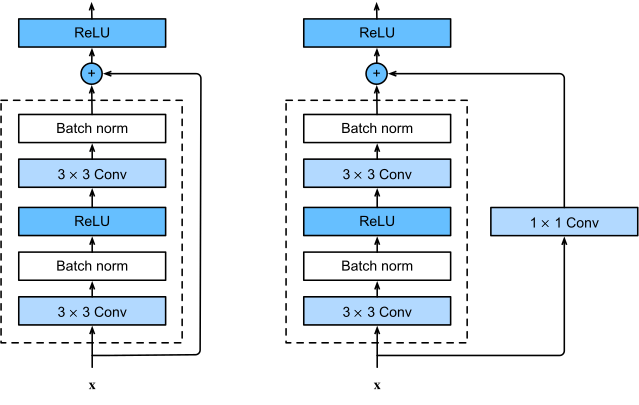
\includegraphics[width=6cm]{plots/moderncnn/resnet-block.png}
    \caption{ResNet block with and without $1 \times 1$ convolution.The information flows through two layers and the identity function. Both streams of information are then element-wise summed and jointly activated (Dive into Deep Learning).}
  \end{figure}

\framebreak
    \begin{itemize}
        \item Let $\mathcal{H}(\xv)$ be the optimal underlying mapping that should be learned by (parts of) the net.
        \item $\xv$ is the input in layer $l$ (can be raw data input or the output of a previous layer).
        \item $\mathcal{H}(\xv)$ is the output from layer $l$.
        \item Instead of fitting $\mathcal{H}(\xv)$, the net is ought to learn the residual mapping $\mathcal{F}(\xv):=\mathcal{H}(\xv)-\xv$ whilst $\xv$ is added via the identity mapping.
        \item Thus, $\mathcal{H}(\xv) = \mathcal{F}(\xv) + \xv$, as formulated on the previous slide.
        \item The model should only learn the \textbf{residual mapping} $\mathcal{F}(\xv)$ 
        \item Thus, the procedure is also referred to as \textbf{Residual Learning}.
    \end{itemize}
\framebreak
    \begin{itemize}
        \item The element-wise addition of the learned residuals $\mathcal{F}(\xv)$ and the identity-mapped data $\xv$ requires both to have the same dimensions.
        \item To allow for downsampling within $\mathcal{F}(\xv)$ (via pooling or valid-padded convolutions), the authors introduce a linear projection layer $W_s$ .
        \item $W_s$ ensures that $\xv$ is brought to the same dimensionality as $\mathcal{F}(\xv)$ such that:
        $$
            y = \mathcal{F}(\xv) + W_s\xv,
        $$
        \item $y$ is the output of the skip module and $W_s$ represents the weight matrix of the linear projection (\# rows of $W_s$ = dimensionality of $\mathcal{F}(\xv)$).
        \item This idea applies to fully connected layers as well as to convolutional layers.
    \end{itemize}
\end{vbframe}

  \framebreak


\begin{vbframe}{ResNet Architecture}
    \begin{itemize}
        \item The residual mapping can learn the identity function more easily, such as pushing parameters in the weight layer to zero.
        \item We can train an effective deep neural network by having residual blocks.
        \item Inputs can forward propagate faster through the residual connections across layers.
        \item ResNet had a major influence on the design of subsequent deep neural networks, both for convolutional and sequential nature.
    \end{itemize}
    
     \begin{figure}
  \centering
    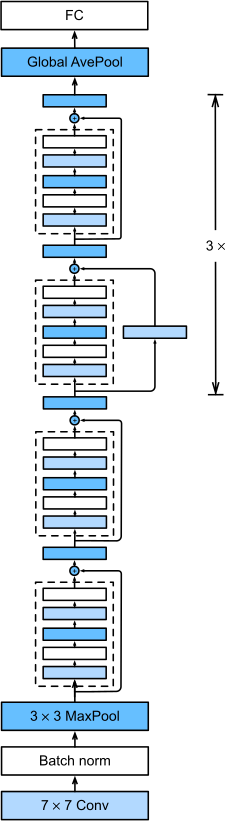
\includegraphics[width=2cm]{plots/moderncnn/resnet18.png}
    \caption{The ResNet-18 architecture (Dive into Deep Learning).}
  \end{figure}
  
 \end{vbframe}

%%%%%%%%%%%%%%%%%%%%%%%%%%%%%%%%%%%%%%%%%%%%%%%%%%%%%%%%%%%%%%%%%%
\section{Densely Connected Networks (DenseNet)}

%\subsection{Dense Blocks}
\begin{vbframe}{From ResNet to DenseNet}
    \begin{itemize}
        \item ResNet significantly changed the view of how to parametrize the functions in deep networks. 
        \item DenseNet (dense convolutional network) is to some extent the logical extension of this [Huang et al., 2017]. 
        \item Dense blocks where each layer is connected to every other layer in feedforward fashion.
        \item Alleviates vanishing gradient, strengthens feature propagation, encourages feature reuse.
        \item To understand how to arrive at it, let us take a small detour to mathematics: 
        \begin{itemize}
             \item Recall the Taylor expansion for functions. For the point  $x=0$  it can be written as: $f(x) = f(0) + f'(0) x + \frac{f''(0)}{2!}  x^2 + \frac{f'''(0)}{3!}  x^3 + \ldots.$
             \item The key point is that it decomposes a function into increasingly higher order terms. In a similar vein, ResNet decomposes functions into : $f(\mathbf{x}) = \mathbf{x} + g(\mathbf{x}).$
             \item That is, ResNet decomposes  f  into a simple linear term and a more complex nonlinear one. What if we want to capture (not necessarily add) information beyond two terms? One solution was DenseNet [Huang et al., 2017].
        \end{itemize}
    \end{itemize}
    
     \begin{figure}
  \centering
    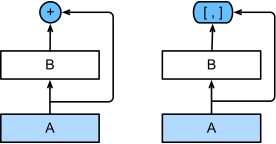
\includegraphics[width=4cm]{plots/moderncnn/densenet-block.png}
    \caption{ DensNet Block (Dive into Deep Learning).}
  \end{figure}
  
\small 
As shown in previous Figure, the key difference between ResNet and DenseNet is that in the latter case outputs are concatenated (denoted by  $[,]$ ) rather than added. As a result, we perform a mapping from  $x$  to its values after applying an increasingly complex sequence of functions:

\vspace{0.2cm}
$\mathbf{x} \to \left[ \mathbf{x}, f_1(\mathbf{x}), f_2([\mathbf{x}, f_1(\mathbf{x})]), f_3([\mathbf{x}, f_1(\mathbf{x}), f_2([\mathbf{x}, f_1(\mathbf{x})])]), \ldots\right].$

\vspace{0.2cm}
\small
In the end, all these functions are combined in MLP to reduce the number of features again. In terms of implementation this is quite simple: rather than adding terms, we concatenate them. 
\newline
The name DenseNet arises from the fact that the dependency graph between variables becomes quite dense. The last layer of such a chain is densely connected to all previous layers. 

\vspace{-0.4cm}
  \begin{figure}
    \centering
    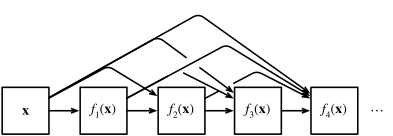
\includegraphics[width=4cm]{plots/moderncnn/densenet.png}
    \caption{The DensNet architecture (Dive into Deep Learning).}
  \end{figure}
  
 \end{vbframe}
 \section{U-Net}
\begin{vbframe}{U-Net}

      \begin{itemize}
        \item U-Net is a fully convolutional net that makes use of upsampling (via transposed convolutions, for example) as well as skip connections.
        \item Input images are getting convolved and down-sampled in the first half of the architecture.
        \item Then, they are getting upsampled and convolved again in the second half to get back to the input dimension.
%        \item Skip connections throughout the net ensure that high-level features from the start can be combined with low-level features throughout the architecture.
        \item Skip connections throughout the net combine feature maps from earlier layers with those from later layers by concatenating both sets of maps along the depth/channel axis.
        \item Only convolutional and no dense layers are used.
    \end{itemize}
\framebreak
    \begin{figure}
        \centering
        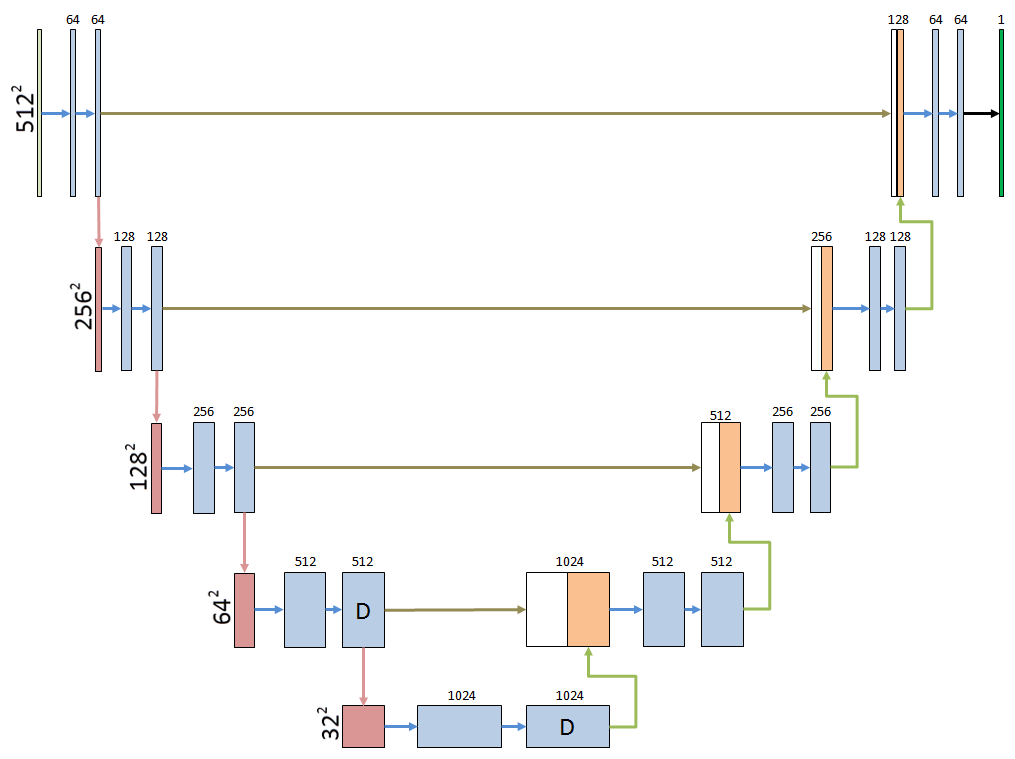
\includegraphics[width=7cm]{plots/outlook/unet.png}
        \caption{Illustration of the architecture. Blue arrows are convolutions, red arrows max-pooling operations, green arrows upsampling steps and the brown arrows merge layers with skip connections. The height and width of the feature blocks are shown on the vertical and the depth on the horizontal. D are dropout layers.}
    \end{figure}
    
\end{vbframe}


\begin{vbframe}{U-Net}

    \begin{itemize}
        \item Example problem setting: train a neural net to pixelwise segment roads in satellite imagery.
        \item Answer the question: \textbf{Where is the road map?}
    \end{itemize}
    \begin{figure}
        \centering
        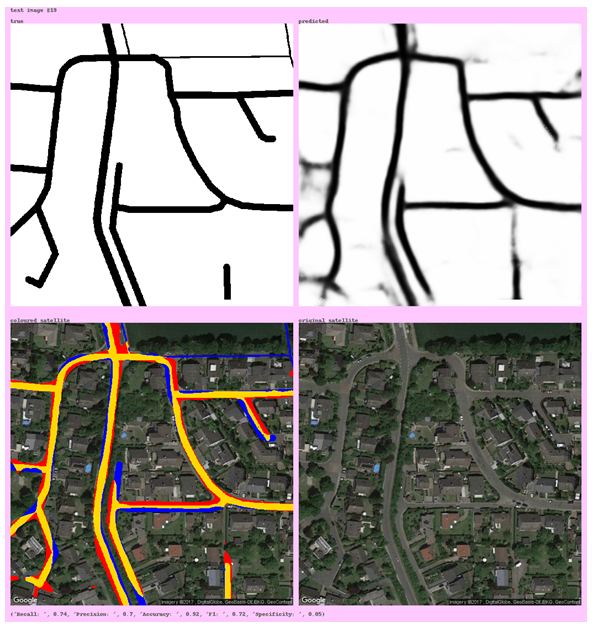
\includegraphics[width=3.8cm]{plots/outlook/31.png}
        \caption{Model prediction on a test satellite image. Yellow are correctly identified pixels, blue false negatives and red false positives.}
    \end{figure}
\framebreak
    \begin{itemize}
        \item The net takes an RGB image [512, 512, 3] and outputs a binary (road / no road) probability mask [512, 512, 1] for each pixel.
        \item The model is trained via a binary cross entropy loss which was combined over each pixel.
    \end{itemize}

  \begin{figure}
        \centering
        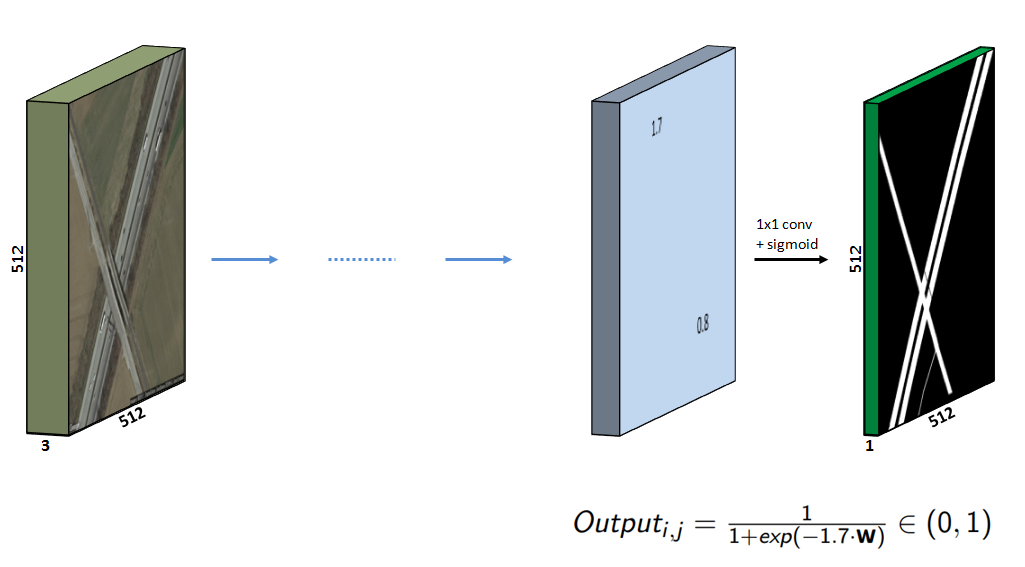
\includegraphics[width=8cm]{plots/outlook/architecture_4.png}
        \caption{Scheme for the input/ output of the net architecture.}
    \end{figure}
    
    

\end{vbframe}



%%%%%%%%%%%%%%%%%%%%%%%%%%%%%%%%%%%%%%%%%%%%%%%%%%%%%%%%%%%%%%%%%%
%%%%%%%%%%%%%%%%%%%%%%%%%%%%%%%%%%%%%%%%%%%%%%%%%%%%%%%%%%%%%%%%%%

%%%%%%%%%%%%%%%%%%%%%%%%%%%%%%%%%%%%%%%%%%%%%%%%%%%%%%%%%%%%%%%%%%
%%%%%%%%%%%%%%%%%%          REFERENCES          %%%%%%%%%%%%%%%%%%
%%%%%%%%%%%%%%%%%%%%%%%%%%%%%%%%%%%%%%%%%%%%%%%%%%%%%%%%%%%%%%%%%%
\begin{vbframe}
\frametitle{References}
\footnotesize{
\begin{thebibliography}{99}

\bibitem[(Dive into Deep Learning)]{1} Dive into Deep Learning . (n.d.-a). \textit{8.4. Multi-branch networks (googlenet)}. \url{http://d2l.ai/chapter_convolutional-modern/googlenet.html}

\bibitem[(Dive into Deep Learning)]{2} Dive into Deep Learning . (n.d.-b). \textit{8.6. Residual Networks (ResNet) and ResNeXt}. \url{http://d2l.ai/chapter_convolutional-modern/resnet.html}

\bibitem[(Dive into Deep Learning)]{3} Dive into Deep Learning . (n.d.-c). \textit{8.7. Densely Connected Networks (DenseNet)
}. \url{http://d2l.ai/chapter_convolutional-modern/densenet.html}

% % \bibitem[Ronneberger et al., 2015]{12} Olaf Ronneberger, Philipp Fischer, Thomas Brox (2015)
% % \newblock U-Net: Convolutional Networks for Biomedical Image Segmentation
% % \newblock \emph{\url{http://arxiv.org/abs/1505.04597}}
% % %%%%%%%%%%%%%%%%%%%%%%%%%%%%%%%%%%
% \bibitem[Zhou et. al , 2016]{25} B. Zhou, Khosla, A., Labedriza, A., Oliva, A. and A. Torralba (2016)
% \newblock Deconvolution and Checkerboard Artifacts
% \newblock \emph{\url{http://cnnlocalization.csail.mit.edu/Zhou_Learning_Deep_Features_CVPR_2016_paper.pdf}}
% %%%%%%%%%%%%%%%%%%%%%%%%%%%%%%%%%%
% %%%%%%%%%%%%%%%%%%%%%%%%%%%%%%%%%%
% \bibitem[Szegedy et. al , 2014]{26} Christian Szegedy, Wei Liu, Yangqing Jia, Pierre Sermanet, Scott Reed, Dragomir Anguelov, Dumitru Erhan, Vincent Vanhoucke and Andrew Rabinovich (2014)
% \newblock Going deeper with convolutions
% \newblock \emph{\url{https://arxiv.org/abs/1409.4842}}
% %%%%%%%%%%%%%%%%%%%%%%%%%%%%%%%%%%
% %%%%%%%%%%%%%%%%%%%%%%%%%%%%%%%%%%
% % \bibitem[Jie Hu et. al , 2014]{27} Jie Hu, Shen, Li and Gang Sun (2017)
% % \newblock Squeeze-and-Excitation Networks
% % \newblock \emph{\url{https://arxiv.org/abs/1709.01507}}
% %%%%%%%%%%%%%%%%%%%%%%%%%%%%%%%%%%
% %%%%%%%%%%%%%%%%%%%%%%%%%%%%%%%%%%
% % \bibitem[Szegedy Christian et. al , 2015]{28} Christian Szegedy, Vanhoucke, Vincent, Sergey, Ioffe, Shlens, Jonathan and Wojna Zbigniew (2015)
% % \newblock Rethinking the Inception Architecture for Computer Vision
% % \newblock \emph{\url{https://arxiv.org/abs/1512.00567}}
% %%%%%%%%%%%%%%%%%%%%%%%%%%%%%%%%%%
% %%%%%%%%%%%%%%%%%%%%%%%%%%%%%%%%%%
% \bibitem[He et. al , 2015]{29} Kaiming He, Zhang, Xiangyu, Ren, Shaoqing, and Jian Sun (2015)
% \newblock Deep Residual Learning for Image Recognition
% \newblock \emph{\url{https://arxiv.org/abs/1512.03385}}
% %%%%%%%%%%%%%%%%%%%%%%%%%%%%%%%%%%
% %%%%%%%%%%%%%%%%%%%%%%%%%%%%%%%%%%
% \bibitem[Zhou et. al, 2016]{32} Bolei Zhou, Aditya Khosla, Agata Lapedriza, Aude Oliva and Antonio Torralba (2016)
% \newblock Learning Deep Features for Discriminative Localization
% \newblock \emph{\url{http://cnnlocalization.csail.mit.edu/Zhou_Learning_Deep_Features_CVPR_2016_paper.pdf}}
% \bibitem[Ronneberger et al., 2015]{12} Olaf Ronneberger, Philipp Fischer, Thomas Brox (2015)
% \newblock U-Net: Convolutional Networks for Biomedical Image Segmentation
% \newblock \emph{\url{http://arxiv.org/abs/1505.04597}}
% 
% %%%%%%%%%%%%%%%%%%%%%%%%%%%%%%%%%%
% %%%%%%%%%%%%%%%%%%%%%%%%%%%%%%%%%%



\end{thebibliography}
}
\end{vbframe}
%%%%%%%%%%%%%%%%%%%%%%%%%%%%%%%%%%%%%%%%%%%%%%%%%%%%%%%%%%%%%%%%%%
%%%%%%%%%%%%%%%%%%%%%%%%%%%%%%%%%%%%%%%%%%%%%%%%%%%%%%%%%%%%%%%%%%
\endlecture
\end{document}
